\documentclass[tikz,border=10pt]{standalone}
\usetikzlibrary{arrows.meta, positioning, calc, backgrounds}

\begin{document}
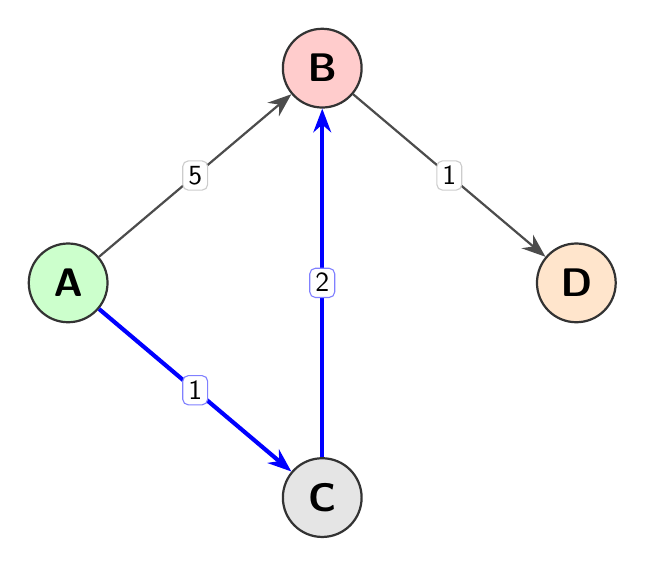
\begin{tikzpicture}[
    node distance=2cm and 2.5cm,
    vertex/.style={circle, draw=black!80, thick, minimum size=10mm, font=\sffamily\Large\bfseries},
    edge/.style={->, >={Stealth[length=3mm]}, thick, draw=black!70},
    highlight_edge/.style={->, >={Stealth[length=3mm]}, line width=1.5pt, draw=blue},
    weight/.style={midway, fill=white, font=\sffamily\normalsize, inner sep=2pt, rounded corners=2pt, draw=black!20, thin}
]

    % Define Nodes
    \node[vertex, fill=green!20] (A) {A};
    \node[vertex, fill=red!20]   (B) [above right=of A] {B};
    \node[vertex, fill=gray!20]  (C) [below right=of A] {C};
    \node[vertex, fill=orange!20](D) [below right=of B, above right=of C] {D};

    % Draw Edges
    \draw[edge] (A) -- (B) node[weight] {5};
    \draw[highlight_edge] (A) -- (C) node[weight, draw=blue!50] {1};
    \draw[highlight_edge] (C) -- (B) node[weight, draw=blue!50] {2};
    \draw[edge] (B) -- (D) node[weight] {1};
\end{tikzpicture}
\end{document}